\chapter*{CAPÍTULO 2. Marco teórico y trabajos relacionados}
\addcontentsline{toc}{chapter}{CAPÍTULO 2. Marco teórico y trabajos relacionados}
\setcounter{chapter}{2}
\setcounter{section}{0}
\setcounter{subsection}{0}
\setcounter{subsubsection}{0}
\setcounter{figure}{0}
\setcounter{table}{0}
\renewcommand{\thesection}{\thechapter.\arabic{section}}
\renewcommand{\thesubsection}{\thesection.\arabic{subsection}}
\renewcommand{\thesubsubsection}{\thesubsection.\arabic{subsubsection}}
\makeatletter
\protected@edef\@currentlabel{\thechapter}%
\makeatother
\label{chap:capitulo2}

En este capítulo se presentan las bases conceptuales que sustentan la investigación y los trabajos relacionados identificados mediante una \acrfull{rsl}. En la primera sección se abordan los conceptos clave relacionados con la deuda social, el síndrome de Burnout, el marco de trabajo \gls{scrum} y la \gls{dsr}. En la segunda sección se describe el protocolo de investigación de la RSL, los hallazgos más relevantes y las brechas existentes que motivan la propuesta de \gls{socialscrum}.

% ------- SECCIÓN 1: DEUDA SOCIAL EN EL DESARROLLO DE SOFTWARE -------
\section{Marco teórico}
\subsection{Deuda social en el desarrollo de software}

La \gls{deuda-social} se describe como la acumulación de costos imprevistos, o potenciales costos, en proyectos de software, generando así un conjunto de decisiones sociotécnicas deficientes que resultan de procesos de desarrollo subóptimos \cite{caballero2022communitysmells}. Dicho de otro modo, a medida que se toman decisiones erróneas de manera constante, los efectos negativos de la deuda social en los equipos de desarrollo de software se vuelven más pronunciados, y mientras estas malas decisiones persistan, sus efectos se intensificarán con el tiempo \cite{caballero2021thesis}. Este concepto, que proviene de la sociología —donde originalmente se usaba para explicar cómo las obligaciones sociales pueden afectar las relaciones interpersonales— ha sido adoptado por los investigadores en ingeniería de software para describir fenómenos similares dentro de los equipos de desarrollo y sus organizaciones \cite{caballero2022communitysmells}.

\subsubsection{Analogía y distinción con la deuda técnica}
La deuda social es, en muchos sentidos, análoga a la deuda técnica \cite{tamburri2015insights}. Ambas representan el estado de las organizaciones de software como resultado de decisiones acumuladas —que, si bien pueden ofrecer beneficios a corto plazo— generan un ``interés'' que se manifiesta como costos adicionales a medio y largo plazo \cite{martini2019agiledebt}. No obstante, existe una diferencia fundamental:
\begin{itemize}
    \item La deuda técnica se centra en decisiones técnicas postergadas, como refactorizaciones de código o decisiones arquitectónicas que afectan la calidad del software \cite{caballero2022communitysmells}.
    \item En contraste, la deuda social se enfoca en decisiones sociotécnicas incorrectas que moldean el entorno de trabajo y que influyen directamente en el bienestar, las interacciones sociales y el rendimiento de los desarrolladores \cite{caballero2022communitysmells}, \cite{caballero2021thesis}. Por lo tanto, mientras la deuda técnica se ocupa de la parte técnica del software, la deuda social pone el foco en las ``personas''. Cabe señalar que, de forma recíproca, la deuda social puede ser una causa subyacente de la deuda técnica \cite{caballero2022communitysmells}, \cite{caballero2021thesis}.
\end{itemize}

\subsubsection{Community smells (olores comunitarios)}
La acumulación de deuda social se inicia con una o más decisiones sociotécnicas equivocadas \cite{caballero2022communitysmells}. La presencia de \gls{community-smells} es un indicador clave de que algo no funciona correctamente dentro de los equipos \cite{caballero2022communitysmells}. Estos olores comunitarios son, en esencia, antipatrones sociotécnicos \cite{caballero2022communitysmells}, definidos como ``conjuntos de circunstancias organizacionales y sociales, con relaciones causales implícitas’’ \cite{caballero2022communitysmells}, \cite{tamburri2015insights}. Cuando estos olores comunitarios persisten, se genera una acumulación de deuda social \cite{caballero2022communitysmells}. Las fuentes identificadas de estos olores comunitarios son diversas y se manifiestan a través de modelos de causa y efecto, por ejemplo:
\begin{itemize}
    \item Decisiones inadecuadas de gestión de la información que resultan en una arquitectura por ósmosis, donde los desarrolladores no tienen acceso a información arquitectónica clave, lo que lleva a la frustración y al desperdicio de tiempo \cite{caballero2022communitysmells}.
    \item Problemas de coordinación de tareas en equipos aislados, conocidos como \gls{cs-org-silo}, que dificultan la comunicación y la cooperación efectiva \cite{caballero2022communitysmells}.
    \item Comportamientos individuales desafiantes, como el \gls{cs-lone-wolf} donde un desarrollador trabaja de forma independiente sin comunicarse con sus compañeros, generando decisiones arquitectónicas no sancionadas y retrasos en el proyecto \cite{caballero2022communitysmells}.
    \item Estructuras organizacionales excesivamente formales o complejas que dan lugar al \gls{cs-radio-silence} o \gls{cs-bottleneck}, creando cuellos de botella en la comunicación y retrasos masivos. Dichos olores comunitarios impactan principalmente en las emociones, estresan las interacciones sociales, afectan el rendimiento del equipo y disminuyen la calidad del software \cite{caballero2022communitysmells}.
\end{itemize}

\subsubsection{El impacto de la deuda social en el entorno ágil}
La deuda social tiene un impacto profundo y multifacético en los equipos de desarrollo ágil y sus organizaciones \cite{caballero2022communitysmells}. Entre las consecuencias más notables se incluyen:
\begin{itemize}
    \item Reacciones humanas adversas y un deterioro del bienestar de los individuos \cite{caballero2022communitysmells}.
    \item Relaciones sociales tensas y conflictos entre compañeros de trabajo, lo que afecta la cohesión del equipo \cite{caballero2022communitysmells}.
    \item Bajo rendimiento del equipo y prácticas de trabajo subóptimas que afectan la calidad del software \cite{caballero2022communitysmells}.
    \item Artefactos de software defectuosos y productos de baja calidad que no cumplen con las expectativas del cliente \cite{caballero2022communitysmells}.
    \item El impacto económico no se limita a simples cifras: suele traducirse en gastos inesperados que, en algunos casos, pueden amenazar la continuidad misma del negocio \cite{caballero2022communitysmells}. Esto cobra especial relevancia en entornos de proyectos ágiles a gran escala (LSA), donde diversos equipos autónomos colaboran en pos de un objetivo común. En estos escenarios, la coordinación y una gestión eficaz no son opcionales, sino piezas clave para mantener el rumbo \cite{martini2019agiledebt}. Una alta autonomía de equipo, si no se equilibra con una alineación adecuada, puede llevar a procesos subóptimos que generen deuda social, como duplicación de trabajo o problemas de integración \cite{martini2019agiledebt}. Como documentan Martini \textit{et al.} \cite{martini2019agiledebt}, la deuda social se manifiesta en discusiones sobre autonomía del equipo, la implicación del liderazgo y la comunicación entre equipos.
\end{itemize}

\subsubsection{Desafíos en la medición y gestión de la deuda social}
Pese a su clara importancia, los investigadores aún enfrentan el desafío de expresar los efectos de la deuda social en términos monetarios precisos \cite{caballero2022communitysmells}. Aunque marcos como DAHLIA \cite{caballero2022communitysmells}, \cite{tamburri2019software} han intentado cuantificar la deuda social, principalmente en relación con la ininteligibilidad arquitectónica, se requiere más investigación empírica para generalizar estas medidas a la vasta gama de olores comunitarios \cite{caballero2022communitysmells}. Por lo tanto, las organizaciones necesitan abordar las decisiones sociotécnicas deficientes y ``saldar'' esta deuda social a través de estrategias de gestión que incluyen enfoques organizacionales, marcos, modelos, herramientas y directrices \cite{caballero2022communitysmells}.

% ------- SECCIÓN 2: SÍNDROME DE BURNOUT -------

\subsection{Síndrome de Burnout}

El Síndrome de \Gls{burnout}, descrito inicialmente en 1974 por el psicólogo Herbert Freudenberger \cite{tulili2022burnout}, es un síndrome relacionado con el trabajo que se manifiesta como agotamiento emocional, despersonalización, sobrecarga laboral y una percepción de escasez de logros personales \cite{tulili2022burnout}. Como bien señalan las investigaciones, su alcance trasciende ámbitos específicos —arquitectura, sector educativo, administración pública o ventas— \cite{tulili2022burnout} para manifestarse como un fenómeno epidémico en entornos STEM (Science, Technology, Engineering y Mathematics). Dicho de otro modo, su omnipresencia y sus repercusiones son un factor crítico que obstaculiza el avance profesional y subyace al estrés laboral en los diversos campos en general \cite{tulili2022burnout}.
En la ingeniería de software (SE) y, sobre todo con respecto a la deuda social, el burnout no es una excepción. De hecho, informes recientes, especialmente tras la pandemia de COVID-19, han puesto de manifiesto que más del 80~\% de los desarrolladores encuestados han experimentado o están experimentando alguna forma de burnout \cite{tulili2022burnout}. La Organización Mundial de la Salud (OMS) ha clasificado el burnout como un fenómeno ocupacional en las ediciones 10ª y 11ª de la Clasificación Internacional de Enfermedades (ICD-10, ICD-11), lo que intensifica su gravedad y el reconocimiento de su impacto en la salud mental en el ámbito laboral \cite{tulili2022burnout}.
Los estudios han explorado a fondo las causas y consecuencias del burnout entre los equipos de desarrollo. Las consecuencias fundamentales reportadas del burnout incluyen:
\begin{itemize}
    \item \textbf{Agotamiento:} La sensación de estar abrumado y exhausto de recursos emocionales y físicos \cite{tulili2022burnout}.
    \item \textbf{Cinismo:} Una actitud negativa, hostil y excesivamente distante hacia el trabajo y los compañeros \cite{tulili2022burnout}.
    \item \textbf{Ineficacia profesional:} La percepción de una disminución en la competencia, el logro personal y productividad en el trabajo \cite{tulili2022burnout}.
\end{itemize}
No obstante, al considerar el burnout como un síntoma de ``deuda social’’, nuestra atención se dirige hacia las dinámicas subyacentes y las expectativas tácitas o explícitas no satisfechas dentro de las interacciones humanas y organizacionales. El burnout en la deuda social sí describe fenómenos que encajan con esta interpretación; por ejemplo, las prácticas de comunicación deficientes son una causa recurrente de burnout:
\begin{itemize}
    \item Una menor participación de los empleados en la comunicación organizacional se correlaciona con un mayor agotamiento emocional \cite{tulili2022burnout}.
    \item La apertura a la crítica puede causar burnout si no se maneja adecuadamente, ya que la falta de retroalimentación constructiva puede llevar a la frustración y al agotamiento emocional \cite{tulili2022burnout}.
    \item Los problemas de comunicación entre gerentes y miembros del equipo, así como los desacuerdos entre compañeros, han sido señalados como factores desencadenantes del burnout \cite{tulili2022burnout}.
\end{itemize}
Teniendo en cuenta lo descrito anteriormente, las relaciones tóxicas en equipos de desarrollo son claros detonantes de burnout. Como demuestran estudios recientes, el lenguaje descortés en comunicaciones técnicas (desde ``solicitudes agresivas’’ hasta comentarios despectivos) erosiona la confianza y genera una deuda social acumulada: ese déficit invisible de respeto y apoyo mutuo que pagamos con estrés crónico \cite{tulili2022burnout}.
Paralelamente, factores como sobrecarga laboral, roles ambiguos o tecnoestrés —estrés causado por la tecnología— aíslan a los profesionales, impidiéndoles conectar con sus equipos \cite{tulili2022burnout}. Cuando la presión ahoga la interacción humana, germina el cinismo y la despersonalización —síntomas clave del burnout. Esta desconexión representa otra deuda organizacional: la que se contrae al sacrificar el bienestar por la productividad inmediata \cite{tulili2022burnout}.
El desenlace es amargo: ese profesional agotado que abandona la carrera no solo reduce la productividad, sino que cobra simbólicamente la deuda social acumulada. Su partida es el recordatorio más crudo de que ningún proyecto sobrevive cuando quema a su gente \cite{tulili2022burnout}.

% ------- SECCIÓN 3: SCRUM -------

\subsection{Scrum}
\subsubsection{Definición de Scrum}
Scrum es un marco de trabajo ligero que ayuda a las personas, equipos y organizaciones a generar valor a través de soluciones adaptativas para problemas complejos \cite{schwaber2020scrum}. Concebido originalmente por Takeuchi y Nonaka \cite{takeuchi1986new} como una analogía del rugby para describir equipos multifuncionales que avanzan juntos, Scrum fue formalizado como proceso de desarrollo de software por Schwaber y Sutherland a mediados de la década de 1990 y ha sido actualizado progresivamente hasta la Scrum Guide 2020 \cite{schwaber2020scrum}.

Su arquitectura se basa en equipos reducidos y autogestionados que operan mediante ciclos iterativos denominados \textit{Sprints}, con una duración máxima de un mes, priorizando la entrega incremental de valor. A diferencia de otras metodologías, Scrum no prescribe herramientas técnicas específicas; su esencia radica en proveer un esqueleto mínimo que catalice la colaboración y la mejora progresiva \cite{takeuchi1986new}.

\subsection{Ciencia del Diseño (Design Science Research)}
\label{sec:dsr}

La investigación de la \gls{dsr} es un paradigma de investigación ampliamente reconocido en los sistemas de información y la ingeniería de software, cuyo objetivo central es la creación y evaluación rigurosa de artefactos como modelos, métodos, constructos o instancias, que resuelvan problemas organizacionales identificados \cite{hevner2004designscience}. A diferencia de las ciencias del comportamiento, que buscan describir y explicar fenómenos, la DSR se orienta a \textit{prescribir} soluciones innovadoras, evaluando su utilidad y eficacia mediante procesos iterativos de diseño y validación.

Peffers \textit{et al.} \cite{peffers2007dsrm} proponen un modelo de proceso ampliamente adoptado que estructura la DSR en seis fases: (1) identificación del problema y motivación, (2) definición de los objetivos de la solución, (3) diseño y desarrollo del artefacto, (4) demostración, (5) evaluación, y (6) comunicación de resultados. Una característica clave de este modelo es que la evaluación del artefacto puede realizarse de múltiples formas desde la evaluación conceptual por expertos hasta la experimentación empírica en contextos reales dependiendo del grado de madurez del artefacto y de las restricciones del entorno de investigación.

Wieringa \cite{wieringa2014dsr} amplía esta perspectiva al distinguir entre la validación previa a la implementación y la validación posterior a la implementación en un contexto real. Esta distinción resulta especialmente relevante para la presente investigación, ya que SocialScrum involucra variables sensibles de salud mental y clima laboral, lo que justifica la realización de una validación conceptual rigurosa como paso previo y necesario antes de una intervención empírica en equipos de desarrollo reales.

En el contexto de esta tesis, la DSR proporciona el marco metodológico que guía la construcción y evaluación del artefacto SocialScrum. Las fases ejecutadas (identificación del problema mediante RSL, diseño y construcción del modelo, evaluación mediante juicio de expertos y comunicación de resultados) se corresponden con las etapas del proceso de Peffers \textit{et al.} \cite{peffers2007dsrm}, como se detalla en la Sección~\ref{sec:metodo-investigacion} del Capítulo~\ref{chap:capitulo1}.

\section{Trabajos relacionados}
A continuación, se presentan algunos hallazgos documentados en la \acrfull{rsl} realizada, que identifican las brechas existentes, los objetivos del proyecto y los aportes encontrados. La RSL se llevó a cabo siguiendo el protocolo detallado en \cite{jalali2012systematic} y \cite{palomba2021communitysmells}, que incluye las siguientes actividades: (i) aplicación del enfoque GQM (Goal-Question-Metric) \cite{caldiera1994gqm} y el marco de trabajo S.M.A.R.T (Specific, Measurable, Achievable, Realistic, Time-bound) \cite{Doran1981}, (ii) definición de la estrategia de búsqueda y selección, (iii) realización de la revisión, y (iv) elaboración del informe de la revisión. La RSL completa está disponible en el Anexo A. Este proceso se realizó con el objetivo de recopilar y categorizar la información existente sobre el tema de investigación. A continuación, en la Figura \ref{fig:smart-gqm} se puede observar la secuencia de actividades realizadas para la RSL:

\begin{figure}[!htbp]
    \centering
    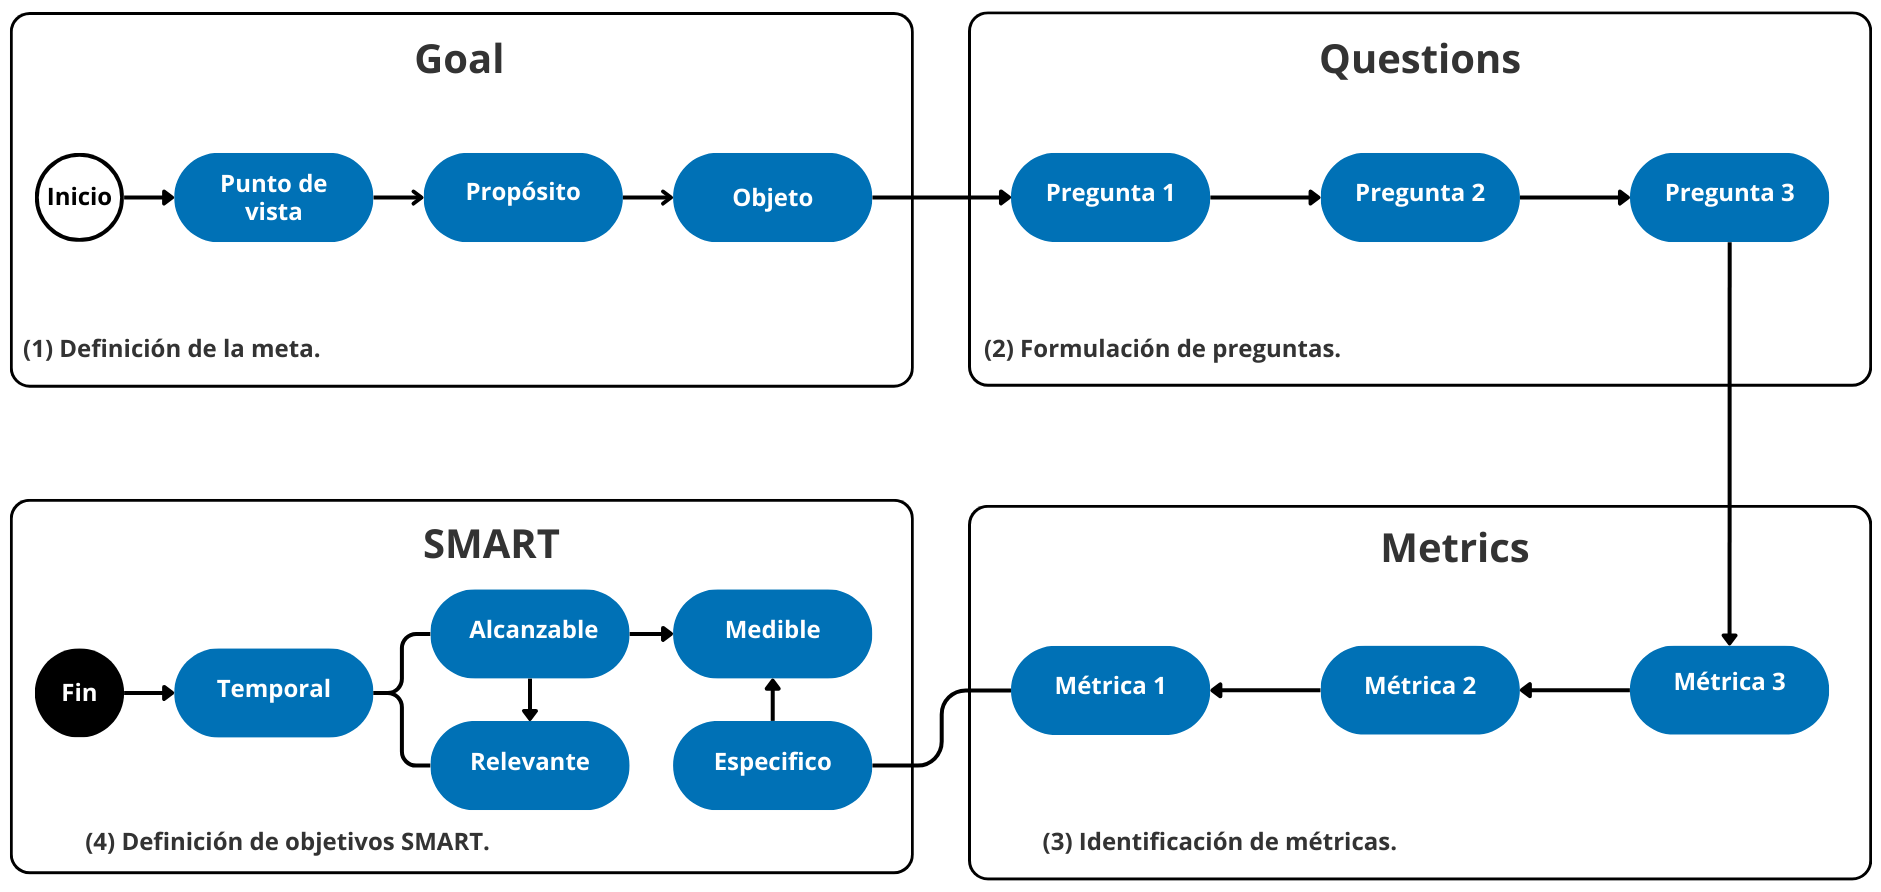
\includegraphics[width=1.0\textwidth]{recursos/capitulo2/smart-gqm.png}
    \caption{Secuencia de actividades realizadas para la RSL}
    \label{fig:smart-gqm}
\end{figure}

\subsection{Protocolo de investigación}
Para llevar a cabo la RSL, se utilizaron herramientas tecnológicas de inteligencia artificial, como ChatGPT \cite{openai2022chatgpt} y Microsoft Copilot \cite{microsoft2023copilot}, con el objetivo de obtener diversas formas de definir un mismo concepto y construir la cadena de búsqueda básica. Los documentos a menudo presentan temas de manera dispersa y poco clara, lo que puede generar sesgos y dudas. En este contexto, las herramientas de IA generativa resultaron ser recursos valiosos, ya que, mediante prompts específicos, permitieron iniciar conversaciones y obtener información más precisa. A partir de los términos identificados con la ayuda de estas herramientas, se definió una versión inicial de la cadena de búsqueda básica: ``social debt'' OR ``social software engineering'' AND ``agile software development'' OR ``software development teams''.
Posteriormente, se seleccionó Google Scholar como la base de datos principal para obtener información o estudios relacionados. Esta elección se basó en varias razones:
\begin{itemize}
    \item Amplia cobertura: Google Scholar indexa una gran variedad de fuentes académicas, incluyendo artículos, tesis, libros y conferencias, lo que permite acceder a una amplia gama de literatura relevante.
    \item Accesibilidad: Es una herramienta de acceso abierto y gratuito, lo que facilita su uso para investigadores con recursos limitados.
    \item Relevancia: Google Scholar utiliza algoritmos que priorizan artículos altamente citados y relevantes, lo que ayuda a identificar estudios influyentes en el campo de la deuda social y el desarrollo ágil.
    \item Integración con otras bases de datos: Aunque Google Scholar fue la base principal, también se complementó con otras bases de datos especializadas, como IEEE Xplore, SpringerLink y Science Direct, para asegurar una revisión exhaustiva.
\end{itemize}
La búsqueda manual reveló que las frases clave ``social debt'' y ``agile software development'' eran esenciales para definir la cadena de búsqueda básica. Por esta razón, se decidió utilizar el conector lógico ``AND'' para unir estas dos frases, ya que los artículos relevantes para la investigación las mencionaban conjuntamente. De esta manera, la cadena de búsqueda básica: ``social debt'' AND ``agile software development'' se aplicó inicialmente a seis bases de datos científicas: Google Scholar, IEEE Xplore, SpringerLink y Science Direct, como se observa en la Tabla \ref{tab:cadenas-busqueda}.

\begingroup
\scriptsize % Fuente ligeramente reducida
\setlength{\LTleft}{0pt} % Alinear tabla a la izquierda
\setlength{\LTright}{0pt} % Permitir que la tabla ocupe espacio a la derecha
\setlength{\tabcolsep}{4pt} % Ajuste de espacio entre columnas
\renewcommand{\arraystretch}{1.4} % Mayor espacio entre filas para facilitar la lectura

\begin{longtable}[H]{|
    >{\Centering\hspace{0pt}}p{0.8cm}|      % Col 1: No.
    >{\RaggedRight\hspace{0pt}}p{9.6cm}|    % Col 2: Cadena de búsqueda 
    >{\Centering\hspace{0pt}}p{2.5cm}|      % Col 3: Fuente 
    >{\Centering\hspace{0pt}}p{2.0cm}|      % Col 4: Estado 
    }

    % --- 1. ENCABEZADO PARA LA PRIMERA PÁGINA ---
    \caption{Cadenas de búsqueda utilizadas en la revisión sistemática} \label{tab:cadenas-busqueda}                                        \\
    \hline
    \textbf{No.} & \textbf{Cadena de búsqueda}                                                          & \textbf{Fuente} & \textbf{Estado} \\
    \hline
    \endfirsthead

    % --- 2. ENCABEZADO PARA PÁGINAS SIGUIENTES ---
    \hline
    \multicolumn{4}{|c|}{{\bfseries \tablename\ \thetable{} -- Continuación}}                                                               \\
    \hline
    \textbf{No.} & \textbf{Cadena de búsqueda}                                                          & \textbf{Fuente} & \textbf{Estado} \\
    \hline
    \endhead

    % --- 3. PIE PARA PÁGINAS INTERMEDIAS ---
    \hline
    \multicolumn{4}{|r|}{\textit{Continúa en la siguiente página...}}                                                                       \\
    \hline
    \endfoot

    % --- 4. PIE FINAL ---
    \hline
    \multicolumn{4}{|l|}{\footnotesize \textit{Acrónimos utilizados: Identificador (No)}}                                                   \\
    \hline
    \endlastfoot

    % --- CONTENIDO ---
    1            & ``social debt'' AND ``agile software development''                                   & Google Scholar  & Incluida        \\
    \hline
    2            & (``Full Text Only'':social debt) AND (``Full Text Only'':agile software development) & IEEE Xplore     & Incluida        \\
    \hline
    3            & ‘‘social debt’ AND ‘agile software development’’                                     & SpringerLink    & Incluida        \\
    \hline
    4            & ‘social debt’ AND ‘agile software development’                                       & Science Direct  & Incluida        \\
\end{longtable}
\endgroup



La cadena de búsqueda se aplicó a una ventana de tiempo desde 2013 hasta 2024, adaptándose a los filtros y parámetros específicos de cada motor de búsqueda. Tras realizar las modificaciones necesarias a la cadena de búsqueda básica, se inició la búsqueda en cada motor. La Tabla \ref{tab:resultados-busqueda-longtable} muestra el total de artículos encontrados, relevantes, repetidos y primarios.

\begingroup
\scriptsize % Fuente ligeramente reducida
\setlength{\LTleft}{0pt} % Alinear tabla a la izquierda
\setlength{\LTright}{0pt} % Permitir que la tabla ocupe espacio a la derecha
\setlength{\tabcolsep}{5pt} % Ajuste de espacio entre columnas
\renewcommand{\arraystretch}{1.4} % Mayor espacio entre filas
\begin{longtable}[H]{|
    >{\Centering\hspace{0pt}}p{0.8cm}|   % Col 1: No.
    >{\RaggedRight\hspace{0pt}}p{4.8cm}| % Col 2: Motor de búsqueda (Aumentado para llenar ancho)
    >{\Centering\hspace{0pt}}p{1.8cm}|   % Col 3: Encontrados
    >{\Centering\hspace{0pt}}p{1.8cm}|   % Col 4: Relevantes
    >{\Centering\hspace{0pt}}p{2.2cm}|   % Col 5: Relevantes repetidos
    >{\Centering\hspace{0pt}}p{2.5cm}|   % Col 6: Primarios seleccionados
    }
    % --- CÁLCULO DE ANCHOS ---
    % Objetivo: ~16.5 - 17cm (Ancho texto A4 típico con márgenes 2.5cm)
    % -------------------------

    % Encabezado primera página
    \caption{Resultados por motor de búsqueda en la revisión sistemática} \label{tab:resultados-busqueda-longtable}                                           \\
    \hline
    \textbf{No.} & \textbf{Motor de búsqueda} & \textbf{Encontrados} & \textbf{Relevantes} & \textbf{Relevantes repetidos} & \textbf{Primarios seleccionados} \\
    \hline
    \endfirsthead

    % Encabezado páginas siguientes
    \hline
    \multicolumn{6}{|c|}{{\bfseries \tablename\ \thetable{} -- Continuación}}                                                                                 \\
    \hline
    \textbf{No.} & \textbf{Motor de búsqueda} & \textbf{Encontrados} & \textbf{Relevantes} & \textbf{Relevantes repetidos} & \textbf{Primarios seleccionados} \\
    \hline
    \endhead

    % Pie páginas intermedias
    \hline
    \multicolumn{6}{|r|}{\textit{Continúa en la siguiente página...}}                                                                                         \\
    \hline
    \endfoot

    % Pie final
    \hline
    \multicolumn{6}{|l|}{\footnotesize \textit{Acrónimos utilizados: Identificador (No)}}                                                                     \\
    \hline
    \endlastfoot

    % CONTENIDO
    1            & Google Scholar             & 130                  & 15                  & 0                             & 8                                \\
    \hline
    2            & IEEE Xplore                & 28                   & 3                   & 0                             & 0                                \\
    \hline
    3            & Science Direct             & 5                    & 0                   & 0                             & 0                                \\
    \hline
    4            & SpringerLink               & 35                   & 2                   & 0                             & 0                                \\
    \hline
                 & \textbf{Total}             & \textbf{198}         & \textbf{20}         & \textbf{0}                    & \textbf{8}                       \\
\end{longtable}
\endgroup


En la Tabla \ref{tab:preguntas-investigacion-longtable} se presentan las preguntas de investigación definidas que ayudaron a segmentar la información identificada en los artículos primarios, su motivación y la relación que tienen con los objetivos propuestos en la RSL. Debido a la limitación de espacio, la RSL se puede consultar en detalle en el Anexo~\ref{anexo:a}.

\begingroup
\scriptsize
\setlength{\LTleft}{0pt} % Alinear tabla a la izquierda
\setlength{\LTright}{0pt} % Permitir que la tabla ocupe espacio a la derecha
\setlength{\tabcolsep}{4pt} % Ajuste de espacio entre columnas
\renewcommand{\arraystretch}{1.4}

\begin{longtable}[H]{|
    >{\Centering\hspace{0pt}}p{0.7cm}|     % Id.
    >{\RaggedRight\hspace{0pt}}p{8.0cm}|   % Pregunta de investigación
    >{\RaggedRight\hspace{0pt}}p{6.5cm}|   % Motivación
    }

    % --- ENCABEZADO PRIMERA PÁGINA ---
    \caption{Preguntas de investigación definidas}
    \label{tab:preguntas-investigacion-longtable}                                                                                                                                                                                                                           \\
    \hline
    \textbf{Id.}                                                                                                                                                                                                 & \textbf{Pregunta de investigación} & \textbf{Motivación} \\
    \hline
    \endfirsthead

    % --- ENCABEZADO PÁGINAS SIGUIENTES ---
    \hline
    \multicolumn{3}{|c|}{{\bfseries \tablename\ \thetable{} -- Continuación}}                                                                                                                                                                                               \\
    \hline
    \textbf{Id.}                                                                                                                                                                                                 & \textbf{Pregunta de investigación} & \textbf{Motivación} \\
    \hline
    \endhead

    % --- PIE PÁGINAS INTERMEDIAS ---
    \hline
    \multicolumn{3}{|r|}{\textit{Continúa en la siguiente página...}}                                                                                                                                                                                                       \\
    \hline
    \endfoot

    % --- PIE FINAL ---
    \hline
    \multicolumn{3}{|l|}{\footnotesize \textit{Acrónimos utilizados: Identificador (Id), Pregunta de investigación (PI)}}                                                                                                                                                   \\
    \hline
    \endlastfoot

    % --- CONTENIDO ---
    PI1                                                                                                                                                                                                          &
    ¿Cuáles son los estudios primarios más citados que han proporcionado según la evidencia aportes importantes e influyentes en el contexto de la gestión de la deuda social en el desarrollo de software ágil? &
    Identificar y evaluar los estudios fundamentales que han tenido un impacto significativo en el campo de la gestión de la deuda social en el desarrollo de software ágil.                                                                                                \\
    \hline

    PI2                                                                                                                                                                                                          &
    ¿Cuál es la distribución de tiempo de publicación de los estudios primarios relevantes con respecto a la deuda social en el desarrollo de software ágil?                                                     &
    Comprender cómo ha evolucionado el interés y el conocimiento sobre la deuda social en el contexto del desarrollo de software ágil a lo largo del tiempo.                                                                                                                \\
    \hline

    PI3                                                                                                                                                                                                          &
    ¿Cuáles son las investigaciones o propuestas desarrolladas cuya idea central sea la gestión de la deuda social en el desarrollo de software ágil hasta la fecha?                                             &
    Identificar y analizar las contribuciones académicas y propuestas prácticas que se han centrado específicamente en la gestión de la deuda social en el desarrollo de software ágil.                                                                                     \\
    \hline

    PI4                                                                                                                                                                                                          &
    ¿Cuáles son los principales desafíos y oportunidades para la investigación futura sobre la deuda social en el desarrollo de software ágil?                                                                   &
    Identificar las barreras y las posibles áreas de crecimiento en el estudio de la deuda social en el desarrollo de software ágil.                                                                                                                                        \\
    \hline

    PI5                                                                                                                                                                                                          &
    ¿Cuáles son las prácticas o enfoques que abordan de manera exitosa la gestión de la deuda social en el desarrollo de software ágil?                                                                          &
    Identificar y evaluar las prácticas y enfoques que han demostrado ser efectivos en la gestión de la deuda social dentro de proyectos de desarrollo de software ágil.                                                                                                    \\
\end{longtable}
\endgroup

A continuación, se presentan las respuestas a algunas de las preguntas que proporcionan información relevante para nuestro análisis. Para más detalles, consulte el Anexo~\ref{anexo:a}, el cual incluye aspectos como: (i) criterios de exclusión e inclusión de los estudios primarios, (ii) criterios de evaluación de calidad, (iii) respuestas a todas las preguntas de investigación, entre otros. En este documento se enfatiza sobre las preguntas de investigación PI4 y PI5 (presentadas en la Tabla 3) por ser consideradas las más relevantes para el lector. Las respuestas a las demás preguntas pueden ser consultadas en el Anexo~\ref{anexo:a}.

\textbf{PI4: ¿Cuáles son los principales desafíos y oportunidades para la investigación futura sobre la deuda social en el desarrollo de software ágil?}

Los principales desafíos en la investigación futura sobre la deuda social en el desarrollo de software ágil incluyen la comprensión de su naturaleza compleja, el desarrollo de métricas efectivas para su evaluación, la integración de enfoques interdisciplinarios y la identificación de estrategias de mitigación. Estos desafíos requieren una profunda comprensión de los aspectos técnicos y sociales involucrados, así como la capacidad de medir y abordar la deuda social de manera oportuna y precisa. Dressen \textit{et al.} \cite{dreesen2021socialdebt} sugieren que actualmente se desconoce qué causa exactamente el aumento de la deuda social y qué mecanismos ayudan a mitigar o disminuir sus efectos adversos. Caballero \textit{et al.} \cite{caballero2022communitysmells} identificaron 30 olores comunitarios, que se analizan mediante un modelo que vincula causas y consecuencias. La información detallada sobre los 30 olores comunitarios se presenta de manera completa en la revisión sistemática de la literatura.

Teniendo en cuenta lo anterior, se presentan las fases que describen cómo surgen los “olores comunitarios” en un equipo de desarrollo de software \cite{caballero2022communitysmells}. Cada fase, desde el inicio del estrés entre los miembros hasta su impacto en la organización y en los usuarios externos, muestra cómo las decisiones sociotécnicas pueden contribuir a la acumulación de deuda social. Las fases del estudio se organizan de la siguiente manera: fase 1, denominada “Inicio”; fase 2, “Impacto directo de los problemas comunitarios”; fase 3, “Difusión del Equipo”; fase 4, “Impacto en la organización”; y, por último, fase 5, “Problemas avanzados”. A continuación, nos enfocaremos en particular en la Fase 3, denominada “Difusión del Equipo”, donde se resalta cómo los miembros que experimentan emociones negativas afectan la cohesión grupal, intensificando así la deuda social. Para un análisis completo de estas fases, se puede consultar la revisión sistemática de la literatura adjuntada en el Anexo A. En este contexto, la intervención de los líderes de proyectos se vuelve esencial. Los líderes no solo deben estar atentos a estos cambios emocionales en sus equipos, sino que también deben ser proactivos en la identificación de estos “olores comunitarios” y en la implementación de estrategias que favorezcan un ambiente de trabajo positivo. Aun así, los líderes de proyectos pueden detectar la presencia de efectos negativos derivados de los “olores comunitarios”. Sin embargo, el desarrollo de un método preciso para diagnosticar, gestionar y solucionar estos problemas depende de la experiencia del líder y de los enfoques de gestión que tenga a su disposición. En este sentido, estos líderes tienen una responsabilidad significativa y una gran oportunidad para prevenir posibles daños organizativos. Al supervisar y mitigar periódicamente los efectos de los olores comunitarios dentro de los equipos de desarrollo de software, pueden contribuir a mantener la cohesión grupal y la calidad del trabajo.

Por otra parte, también se presentan oportunidades para investigar, entre ellas: nuevas tecnologías y herramientas, explorar la relación entre la deuda social y el rendimiento del equipo, estudiar el papel de la cultura organizacional y evaluar el impacto a largo plazo de la deuda social en la dinámica del equipo y la calidad del software. Estas oportunidades pueden conducir a una comprensión más completa de la deuda social en entornos ágiles y al desarrollo de estrategias más efectivas para su gestión y mitigación \cite{saeeda2024multivocal}.

\textbf{PI6: ¿Cuáles son las practicas o enfoques que abordan de manera exitosa la gestión de la deuda social en el desarrollo de software ágil?}

Dressen \textit{et al.} \cite{dreesen2021socialdebt} sugieren una estrategia para abordar la deuda social fundamentada en el modelo de las 3C’s, que enfatiza las deficiencias en comunicación, colaboración y coordinación. El enfoque de mitigación sugerido por Dressen \textit{et al.} \cite{dreesen2021socialdebt} se concentra particularmente en mejorar la comunicación y la colaboración, destacando los siguientes puntos presentados en la Tabla \ref{tab:enfoques_mitigacion}:

\begingroup
\scriptsize
\setlength{\LTleft}{0pt} % Alinear tabla a la izquierda
\setlength{\LTright}{0pt} % Permitir que la tabla ocupe espacio a la derecha
\setlength{\tabcolsep}{4pt} % Ajuste de espacio entre columnas
\renewcommand{\arraystretch}{1.4}

\begin{longtable}{|
    >{\Centering\hspace{0pt}}p{0.7cm}|
    >{\RaggedRight\hspace{0pt}}p{4.0cm}|
    >{\RaggedRight\hspace{0pt}}p{10.5cm}|
    }

    \caption{Enfoques de mitigación de la deuda social en equipos de desarrollo de software ágil distribuido}
    \label{tab:enfoques_mitigacion}                                                                                                                                                                                                                                                                                                                                                                                                                                                                                                                                                                                                                                                                         \\
    \hline
    \textbf{No.}                                                                            & \textbf{Enfoque de mitigación} & \textbf{Descripción}                                                                                                                                                                                                                                                                                                                                                                                                                                                                                                                                                         \\
    \hline
    \endfirsthead

    \hline
    \multicolumn{3}{|c|}{{\bfseries \tablename\ \thetable{} -- Continuación}}                                                                                                                                                                                                                                                                                                                                                                                                                                                                                                                                                                                                                               \\
    \hline
    \textbf{No.}                                                                            & \textbf{Enfoque de mitigación} & \textbf{Descripción}                                                                                                                                                                                                                                                                                                                                                                                                                                                                                                                                                         \\
    \hline
    \endhead

    \hline
    \multicolumn{3}{|r|}{\textit{Continúa en la siguiente página...}}                                                                                                                                                                                                                                                                                                                                                                                                                                                                                                                                                                                                                                       \\
    \hline
    \endfoot

    \hline
    \multicolumn{3}{|l|}{\footnotesize \textit{Acrónimos utilizados: Identificador (No)}}                                                                                                                                                                                                                                                                                                                                                                                                                                                                                                                                                                                                                   \\
    \hline
    \endlastfoot

    1                                                                                       &
    Comunicación honesta y abierta                                                          &
    Es fundamental en equipos de desarrollo de software ágil distribuido para mitigar la deuda social. La comunicación honesta y abierta se define por su franqueza y transparencia, lo que ayuda a construir confianza mutua entre los miembros del equipo. Esta confianza facilita la resolución efectiva de conflictos sociales, ya que los miembros del equipo pueden abordar los problemas directamente. En última instancia, esta comunicación directa contribuye a crear un ambiente de trabajo constructivo y ayuda a reducir la acumulación de deuda social en el equipo.                                                                                                                          \\

    \hline

    2                                                                                       &
    Intensidad de la comunicación relacionada con las tareas                                &
    Se refiere a la naturaleza altamente enfocada y orientada a objetivos de la interacción en el trabajo remoto. Las interacciones y la comunicación no son aleatorias, sino que están determinadas o preparadas de antemano para completar tareas específicas, reduciendo las distracciones. Este enfoque intensificado en la comunicación relacionada con las tareas puede ayudar a mitigar el efecto de los factores que contribuyen a la deuda social en equipos de desarrollo de software ágil distribuido (\gls{asd}).                                                                                                                                                                               \\

    \hline

    3                                                                                       &
    Intensidad de la colaboración relacionada con las tareas con respecto a la colaboración &
    Se refiere a cómo las interacciones durante el trabajo remoto están altamente enfocadas en tareas y objetivos específicos. Esto significa que todas las acciones colaborativas están orientadas a completar la tarea en cuestión, reduciendo las distracciones. Este enfoque intensificado en la colaboración relacionada con las tareas puede tener un efecto tanto en promover como en mitigar la deuda social en equipos de desarrollo de software ágil distribuidos. Por un lado, puede conducir a una comunicación más directa y eficiente, pero por otro, puede resultar en una falta de interacción informal que es importante para la construcción de relaciones y la resolución de conflictos. \\

    \hline

    4                                                                                       &
    Costos iniciales reducidos para iniciar interacciones o comunicaciones                  &
    Se refieren a la capacidad de establecer rápidamente un entorno para la colaboración y comunicación uno a uno sin restricciones. Esto es beneficioso en un contexto de trabajo remoto, ya que las salas de reuniones libres ya no son un recurso escaso y se puede configurar la comunicación sin casi ninguna limitación. Este factor ayuda a mitigar la deuda social en equipos de desarrollo de software ágil distribuido al facilitar la resolución de conflictos y promover una comunicación más directa y abierta entre los miembros del equipo.                                                                                                                                                  \\
\end{longtable}
\endgroup

Por otra parte, Saeeda \textit{et al.} \cite{saeeda2024multivocal} llevaron a cabo un estudio exhaustivo sobre varios tipos de \gls{non-technical-debt}, incluyendo la deuda social, explorando sus causas y proponiendo múltiples estrategias para su mitigación. Identifican que las causas de la deuda social derivan de tres factores principales: limitaciones sociales, desafíos organizacionales y dinámicas comunitarias. A partir de estos factores, se delinean ocho estrategias basadas en evidencias de la literatura científica y gris para reducir la deuda social, como se puede visualizar en la Tabla \ref{tab:estrategias_mitigacion_enfoque} las cuales son:

\begingroup
\scriptsize
\setlength{\LTleft}{0pt} % Alinear tabla a la izquierda
\setlength{\LTright}{0pt} % Permitir que la tabla ocupe espacio a la derecha
\setlength{\tabcolsep}{4pt} % Ajuste de espacio entre columnas
\renewcommand{\arraystretch}{1.4}

\begin{longtable}{|
    >{\Centering\hspace{0pt}}p{0.7cm}|
    >{\RaggedRight\hspace{0pt}}p{4.0cm}|
    >{\RaggedRight\hspace{0pt}}p{10.5cm}|
    }

    \caption{Estrategias de mitigación de la deuda social en equipos de desarrollo de software}
    \label{tab:estrategias_mitigacion_enfoque}                                                                                                                                                                                                                                                                                                                \\
    \hline
    \textbf{No.}                                                                & \textbf{Estrategias de mitigación} & \textbf{Descripción}                                                                                                                                                                                                                   \\
    \hline
    \endfirsthead

    \hline
    \multicolumn{3}{|c|}{{\bfseries \tablename\ \thetable{} -- Continuación}}                                                                                                                                                                                                                                                                                 \\
    \hline
    \textbf{No.}                                                                & \textbf{Estrategias de mitigación} & \textbf{Descripción}                                                                                                                                                                                                                   \\
    \hline
    \endhead

    \hline
    \multicolumn{3}{|r|}{\textit{Continúa en la siguiente página...}}                                                                                                                                                                                                                                                                                         \\
    \hline
    \endfoot

    \hline
    \multicolumn{3}{|l|}{\footnotesize \textit{Acrónimos utilizados: Identificador (No)}}                                                                                                                                                                                                                                                                     \\
    \hline
    \endlastfoot

    1                                                                           &
    \Gls{sna}                                                                   &
    Emplear el análisis de redes para entender mejor la deuda.                                                                                                                                                                                                                                                                                                \\

    \hline

    2                                                                           &
    Comunicación colaborativa                                                   &
    Promover una comunicación efectiva dentro del equipo.                                                                                                                                                                                                                                                                                                     \\

    \hline

    3                                                                           &
    Gestión de la composición del equipo y mejora de decisiones arquitectónicas &
    Establecer directrices claras para la formación de equipos y la toma de decisiones arquitectónicas.                                                                                                                                                                                                                                                       \\

    \hline

    4                                                                           &
    Entornos de trabajo híbridos                                                &
    Fomentar entornos que combinen modalidades presenciales y remotas.                                                                                                                                                                                                                                                                                        \\

    \hline

    5                                                                           &
    Métricas para la comunicabilidad de la arquitectura del software            &
    Desarrollar y aplicar métricas específicas que faciliten la comprensión arquitectónica.                                                                                                                                                                                                                                                                   \\

    \hline

    6                                                                           &
    Marcos de trabajo para la mitigación de la deuda social                     &
    Implementar marcos como CAFFEA, que combina el desarrollo de software ágil con el desarrollo y manejo continuo de la arquitectura de software, especialmente en empresas grandes con líneas de productos complejos.                                                                                                                                       \\

    \hline

    7                                                                           &
    Tácticas arquitectónicas y frameworks sociotécnicos                         &
    El enfoque DAHLIA, que incluye la popularidad y la conciencia en las decisiones, junto con el marco de calidad sociotécnica.                                                                                                                                                                                                                              \\

    \hline

    8                                                                           &
    Herramientas específicas                                                    &
    Introducir herramientas como GEEZMO, que monitorea el estado de ánimo del equipo; CodeFace4Smell, que detecta causas de deuda social en silos organizacionales; y YOSHI (Yielding Open-Source Health Information), que proporciona transparencia y asistencia computacional a las comunidades de software de código abierto \cite{maelstromdat2014yoshi}. \\
\end{longtable}
\endgroup

\subsection{Brechas existentes}

A partir del análisis realizado en la RSL (ver en detalle en el Anexo~\ref{anexo:a}), existen importantes brechas en la comprensión y gestión de la deuda social en el desarrollo de software ágil. Primero, aunque se reconoce la deuda social, hay poca investigación sobre cómo llevar a cabo su gestión en equipos ágiles. En pocas palabras, no se evidenció la definición de un marco claro que permita gestionarla y abordarla de manera sistemática. Además, pese a que se entienden sus impactos, faltan soluciones claras que permitan guiar a las organizaciones en la implementación de estrategias efectivas que culminen con una gestión mucho más sistemática de la deuda social cuando se identifique. El enfoque cortoplacista, que prioriza cumplir plazos y reducir costos, lleva a decisiones que aumentan la deuda social sin equilibrar el bienestar del equipo, y esto se ve impactado en una mayor magnitud si no se sabe cómo gestionar dicha deuda. También faltan herramientas y métricas para evaluar el impacto de la deuda social en la calidad del trabajo y el bienestar del equipo, dificultando su identificación y gestión. Finalmente, la comunicación inadecuada y la falta de colaboración en la toma de decisiones relacionada con la deuda social es consecuencia de la ausencia de una solución que provea los elementos que permitan, de manera sistemática, gestionar la deuda social.

A partir de las brechas identificadas, la literatura evidencia la necesidad de aportar una adaptación de Scrum ---como SocialScrum--- que incorpore mecanismos explícitos para la gestión de la deuda social. En particular, se requiere un enfoque estructurado que integre sesiones de retrospectiva focalizadas en aspectos sociales, ciclos dedicados a la identificación y resolución de conflictos interpersonales, y prácticas de comunicación transparente que fortalezcan la cohesión del equipo. Estos elementos, ausentes en los marcos ágiles convencionales, constituyen la contribución central de esta investigación, cuyo diseño y fundamentación se detallan en los Capítulos~\ref{chap:capitulo3} y \ref{chap:capitulo4}.
